\begin{figure}
    \centering
    \begin{minipage}[t]{0.28\linewidth}
        \centering
        \resizebox{!}{0.25\textheight}{
        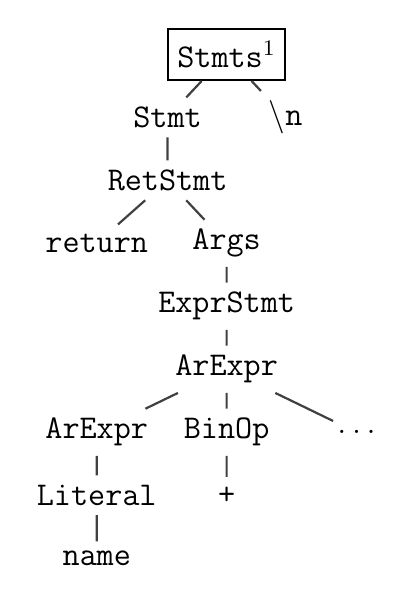
\begin{tikzpicture}
        [font=\large, edge from parent,
        % every node/.style={top color=white, bottom color=black!20,
        % ellipse, minimum size=8mm, draw=black!75,
        % thick, drop shadow, align=center},
        edge from parent/.style={draw=black!75, thick},
        level distance=0.8cm, xscale=1.0]
        \node [style={minimum size=6.5mm, draw=black, thick}] (stmts2) {\texttt{Stmts$^1$}}
        child {
            node (stmt2) {\texttt{Stmt}}
            child {
                node (RetStmt) {\texttt{RetStmt}}
                child [xscale=1.2] {
                    node (return) {\texttt{\bfseries return}}
                }
                child {
                    node (args) {\texttt{Args}}
                    child {
                        node (expr2) {\texttt{ExprStmt}}
                        child [xscale=1.1] {
                            node (arexpr1) {\texttt{ArExpr}}
                            child {
                                node (arexpr2) {\texttt{ArExpr}}
                                child {
                                    node (literal) {\texttt{Literal}}
                                    child {
                                        node (name3) {\texttt{name}}
                                    }
                                }
                            }
                            child {
                                node (binop) {\texttt{BinOp}}
                                child {
                                    node (plus) {\texttt{\bfseries +}}
                                }
                            }
                            child {
                                node (empty) {\texttt{$\dots$}}
                            }
                        }
                    }
                }
            }
        }
        child {
            node (newline3) {\texttt{\textbackslash n}}
        };
        \end{tikzpicture}
        } \subcaption{The partial parse tree for the example at
        \autoref{fig:bad-prog}.}
        \label{fig:partial-parse-tree-2}
    \end{minipage}
    \hspace{0.02\linewidth}%
    \begin{minipage}[t]{0.35\linewidth}
        \centering
        \hspace*{0.04\linewidth}%
        \resizebox{!}{0.25\textheight}{
            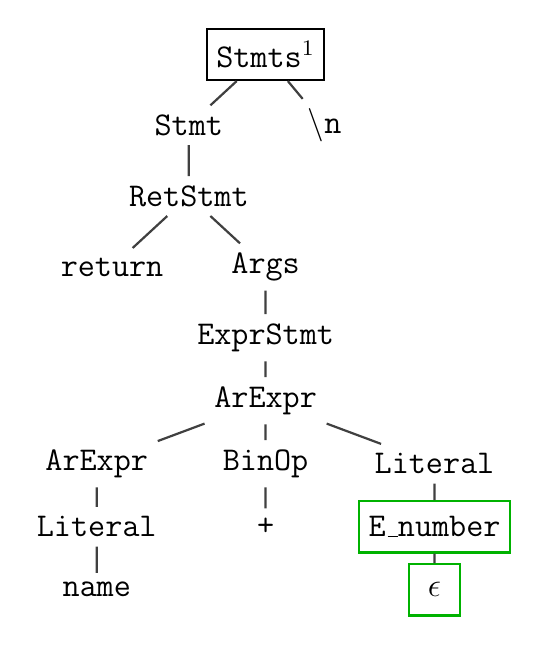
\begin{tikzpicture}
            [font=\large, edge from parent,
            % every node/.style={top color=white, bottom color=black!20,
            % ellipse, minimum size=8mm, draw=black!75,
            % thick, drop shadow, align=center},
            edge from parent/.style={draw=black!75, thick},
            level distance=0.9cm, xscale=1.0]
            \node [style={minimum size=6.5mm, draw=black, thick}] (stmts2) {\texttt{Stmts$^1$}}
            child [xscale=1.3] {
                node (stmt2) {\texttt{Stmt}}
                child {
                    node (RetStmt) {\texttt{RetStmt}}
                    child {
                        node (return) {\texttt{\bfseries return}}
                    }
                    child {
                        node (args) {\texttt{Args}}
                        child {
                            node (expr2) {\texttt{ExprStmt}}
                            child [level distance=0.8cm, xscale=1.1] {
                                node (arexpr1) {\texttt{ArExpr}}
                                child {
                                    node (arexpr2) {\texttt{ArExpr}}
                                    child {
                                        node (literal1) {\texttt{Literal}}
                                        child {
                                            node (name3) {\texttt{name}}
                                        }
                                    }
                                }
                                child {
                                    node (binop) {\texttt{BinOp}}
                                    child {
                                        node (plus) {\texttt{\bfseries +}}
                                        }
                                }
                                child {
                                    node (literal2) {\texttt{Literal}}
                                    child {
                                        node [style={minimum size=6.5mm, draw=black!30!green, thick}] (enumber) {\texttt{E\_number}}
                                        child {
                                            node [style={minimum size=6.5mm, draw=black!30!green, thick}] (eps) {\texttt{$\epsilon$}}
                                        }
                                    }
                                }
                            }
                        }
                    }
                }
            }
            child {
                node (newline3) {\texttt{\textbackslash n}}
            };
            \end{tikzpicture}
        } \subcaption{Adding a number with the green \texttt{E\_number} error rule.}
        \label{fig:adding-partial}
    \end{minipage}
    \hspace{0.01\linewidth}%
    \begin{minipage}[t]{0.32\linewidth}
        \centering
        \resizebox{!}{0.25\textheight}{
            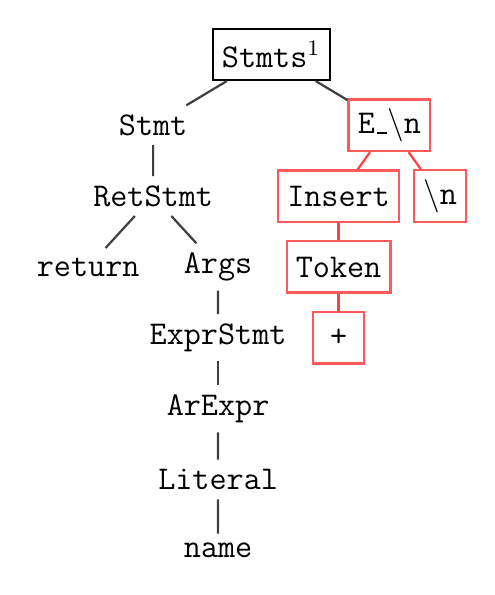
\begin{tikzpicture}
            [font=\large, edge from parent,
            % every node/.style={top color=white, bottom color=black!20,
            % ellipse, minimum size=8mm, draw=black!75,
            % thick, drop shadow, align=center},
            edge from parent/.style={draw=black!75, thick},
            level distance=0.9cm, xscale=2.0]
            \node [style={minimum size=6.5mm, draw=black, thick}] (stmts2) {\texttt{Stmts$^1$}}
            child {
                node (stmt2) {\texttt{Stmt}}
                child [xscale=0.55] {
                    node (RetStmt) {\texttt{RetStmt}}
                    child {
                        node (return) {\texttt{\bfseries return}}
                    }
                    child {
                        node (args) {\texttt{Args}}
                        child {
                            node (expr2) {\texttt{ExprStmt}}
                            child {
                            node (arexpr1) {\texttt{ArExpr}}
                                child {
                                    node (literal1) {\texttt{Literal}}
                                    child {
                                        node (name3) {\texttt{name}}
                                    }
                                }
                            }
                        }
                    }
                }
            }
            child {
                node [style={minimum size=6.5mm, draw=red!65, thick}] (enewline) {\texttt{E\_\textbackslash n}}
                child [edge from parent/.style={draw=red!75, thick}, xscale=0.43] {
                    node [style={minimum size=6.5mm, draw=red!65, thick}] (insert) {\texttt{Insert}}
                    child {
                        node [style={minimum size=6.5mm, draw=red!65, thick}] (token) {\texttt{Token}}
                        child {
                            node [style={minimum size=6.5mm, draw=red!65, thick}] (plus) {\texttt{\bfseries +}}
                        }
                    }
                }
                child [edge from parent/.style={draw=red!75, thick}, xscale=0.43] {
                    node [style={minimum size=6.5mm, draw=red!65, thick}] (newline3) {\texttt{\textbackslash n}}
                }
            };
            \end{tikzpicture}
        }
        \subcaption{Deleting the \texttt{+} with red \texttt{E\_\textbackslash n} error rule.}
        \label{fig:deleting-partial}
    \end{minipage}
    \caption{The rest of the problematic function in
    \autoref{fig:partial-parse-tree-1} and two possible error correcting parses}
    \label{fig:two-partial-parses}
\end{figure}
